\section{Validierung}
In diesem Kapitel wird zuerst der Versuchsaufbau erklärt. Danach werden die einzelnen Versuche und deren Erkenntnis erläutert.

\subsection{Versuchsaufbau}
Für den Versuchsaufbau wurde BLDC-Motor mit einer asynchronen Maschine gekoppelt welche über einen Frequenzumrichter angesteuert wird. Die asynchrone Maschine dient bei diesen Versuche als Last.


\subsection{Drehmoment bei variabler Drehzahl}
Bei diesem ersten Versuch gilt es zu verifizieren, ob der BLDC-Motor das erforderliche Drehmoment unabhängig von der Drehzahl erreichen kann.

% dieser Teil eventulle in den Hartwareteil verschieben und nur darauf Referenzieren
Bei einem minimalen mechanischen Wirkungsgrad von 0.8, einem 1:16 Getriebe und einem Trommeldurchmesser von 80cm, muss der Motor ein konstantes Drehmoment von 32Nm liefern.

Das Drehmoment an der Welle des BLDC-Motors wird mithilfe der Formel (FORMEL IN HARWARE/GRUNDLAGEN) über die Leistung und der Drehzahl des Motors ermittelt. Diese Kurve ist in der Abbildung \ref{fig:drehmoment/drehzahl} (blaue Kurve) ersichtlich. Da die asynchrone Maschine ebenfalls nicht ideal arbeitet, wird bei dieser einen Wirkungsgrad von 90\% angenommen (rote Kurve). 

\begin{figure}[H]
	\centering
	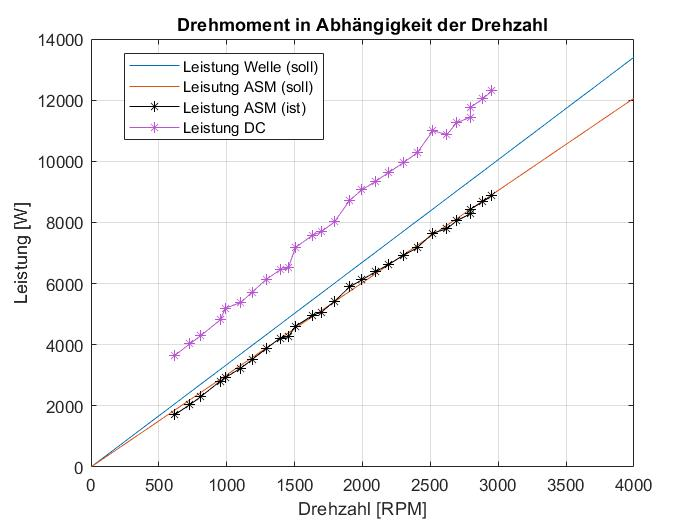
\includegraphics[width=0.8\linewidth]{drehmoment_drehzahl.jpg}
	\caption{Drehmoment in Abhängigkeit der Drehzahl}\label{fig:drehmoment/drehzahl}
\end{figure}

Bei diesem Versuch ist ersichtlich, dass es möglich war, die erforderliche Leistung (schwarze Punkte) im Drehzahlbereich zwischen 600 und 3000 RPM zu erreichen. Die aufgenommene Leistung auf der DC-Seite (violette Punkte) ist dabei proportional zur abgegebenen Leistung angestiegen.

In der Abbildung \ref{fig:drehmoment/StromSpannung} sind die Spannung, der Strom und die Sollwertvorgabe für die Ansteuerung während des Versuchs ersichtlich. Die Spannung wurde nachgeregelt (blaue Punkte), damit diese konstant bleibt. Der Strom (rote Punkte) und der Sollwert für die Ansteuerung (orange Punkte) wurden ebenfalls während des Versuchs dokumentiert.

\begin{figure}[H]
	\centering
	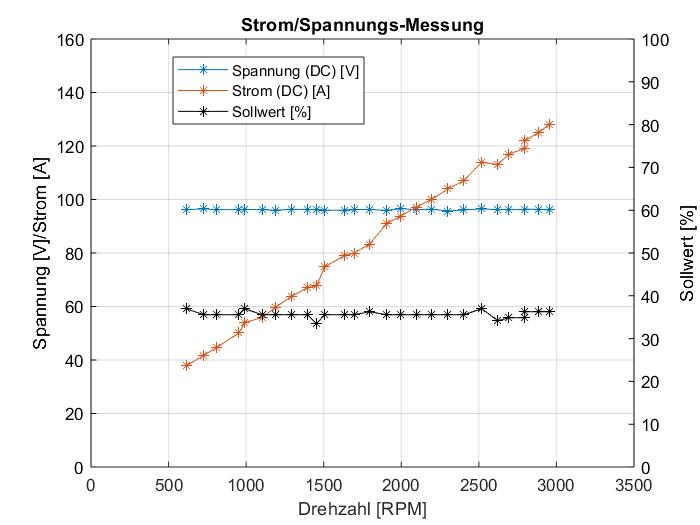
\includegraphics[width=0.8\linewidth]{drehmoment_StromSpannung.jpg}
	\caption{Spannung und Strom während des Drehmomentversuchs}\label{fig:drehmoment/StromSpannung}
\end{figure}

Da der graue Transformator nur für einen Strom von 95A konzipiert ist, was einem Strom von ca. 128A im DC-Zwischenkreis entspricht, konnte der Versuch nicht bis 3800 RPM durchgeführt werden. Der Strom kann mit guter Näherung als linear zur Drehzahl bei gleichbleibendem Drehmoment betrachtet werden. Dadurch ist ersichtlich, dass bei 3800 RPM ein Strom von ca. 160A benötigt wird. Dies Stromstärke deckt sich auch mit dem, was im Datenblatt des Motors angegeben wird (REFERENZ AUF DATENBLATT).

Bei diesem Versuch ist ebenfalls ersichtlich, dass die Sollwertvorgabe über den Drehzahlbereich nur kleine Abweichungen hat und daher in guter Näherung als konstant betrachtet werden kann.


\subsection{Leistungsverhalten bei Spannungsabfall}
Bei diesem Versuch wird das Verhalten des Controllers bei einem Spannungsabfall untersucht. Dabei wurde die Leistung der asynchronen Maschine (rechte Abbildung) und der Strom (linke Abbildung) des Controllers in Abhängigkeit der Spannung des Controllers gemessen. Der Sollwert wurde während des gesamten Versuchs konstant auf 35.5\% gehalten. Dieser Versuch wurde zuerst mit 1500 RPM (blaue Punkte) und danach nochmals mit 2000 RPM (rote Punkte) durchgeführt.

\begin{figure}[H]
	\centering
	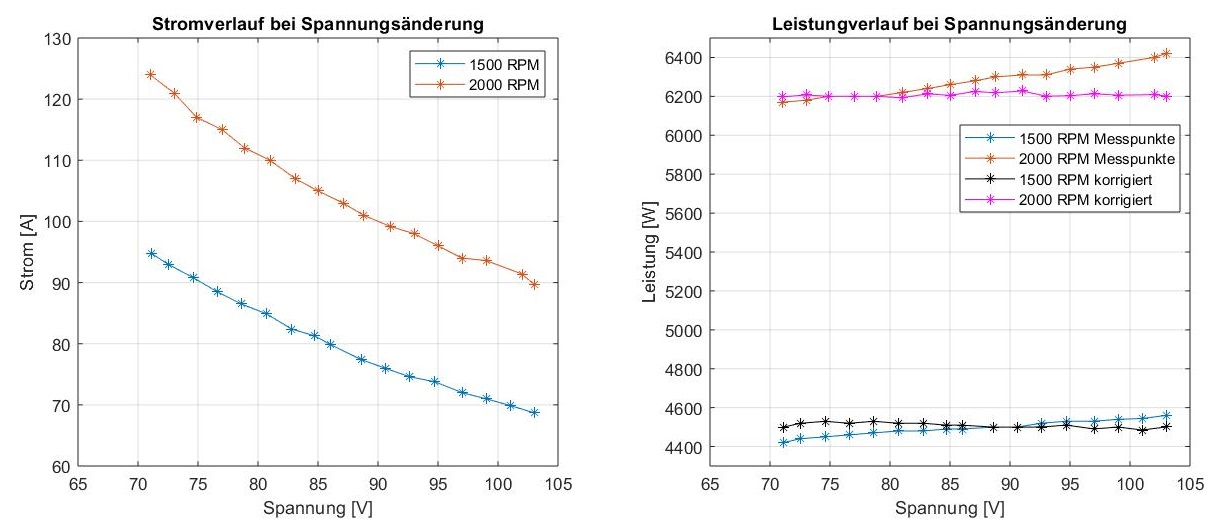
\includegraphics[width=1\linewidth]{Spannungsversuch.jpg}
	\caption{Leistungs- und Stromverlauf bei Spannungsabfall}\label{fig:Spannungsabfall}
\end{figure}
